%% General definitions
\documentclass{article} %% Determines the general format.
\usepackage{a4wide} %% paper size: A4.
\usepackage[utf8]{inputenc} %% This file is written in UTF-8.
%% Some editors on Windows cannot save files in UTF-8.
%% If there is a problem with special characters not showing up
%% correctly, try switching "utf8" to "latin1" (ISO 8859-1).
\usepackage[T1]{fontenc} %% Format of the resulting PDF file.
\usepackage{fancyhdr} %% Package to create a header on each page.
\usepackage{lastpage} %% Used for "Page X of Y" in the header.
                      %% For this to work, you have to call pdflatex twice.
\usepackage{enumerate} %% Used to change the style of enumerations (see below).

\usepackage{amssymb} %% Definitions for math symbols.
\usepackage{amsmath} %% Definitions for math symbols.

\usepackage{tikz}  %% Pagacke to create graphics (graphs, automata, etc.)
\usetikzlibrary{shapes,arrows,calc,positioning}
\usetikzlibrary{graphs}
\usetikzlibrary{automata} %% Tikz library to draw automata
\usetikzlibrary{arrows}   %% Tikz library for nicer arrow heads
\usetikzlibrary{positioning}    %% Tikz library for more positioning options

\usepackage{hyperref} %% hyperlinks

\usepackage{chessfss} % contained in debian package texlive-games

\usepackage{listings}   % include & display python code
\usepackage[edges]{forest}  % for search trees

\tikzset{WhiteSquare/.style = {shape=rectangle, minimum width=28, minimum
    height=28, anchor=south west}}
\tikzset{BlackSquare/.style = {shape=rectangle, fill=lightgray, minimum
    width=28, minimum height=28, anchor=south west}}

%% Left side of header
\lhead{\course\\\semester\\Exercise \homeworkNumber}
%% Right side of header
\rhead{\authorname\\Page \thepage\ of \pageref{LastPage}}
%% Height of header
\usepackage[headheight=36pt]{geometry}
%% Page style that uses the header
\pagestyle{fancy}

%% Triangle node definitions (tikzpicture)
\tikzset{
    triangleup/.style={
        regular polygon,
        regular polygon sides=3,
        draw,
        shape border rotate=0,
        align=center,
        minimum size=8mm
    },
    triangledown/.style={
        regular polygon,
        regular polygon sides=3,
        draw,
        shape border rotate=180,
        align=center,
        minimum size=8mm
    }
}

\newcommand{\authorname}{Benjamin Regez\\Luis Tritschler}
\newcommand{\semester}{Spring Semester 2026}
\newcommand{\course}{Foundations of Artificial Intelligence}
\newcommand{\homeworkNumber}{11}

\renewcommand{\thesection}{Exercise \homeworkNumber.\arabic{section}}


\begin{document}

\section{}
\begin{enumerate}[(a)]
    \item $\mathcal{S} = \langle S, A, T, s_I, S_G,
    \textit{utility}, \textit{player} \rangle$ with
    \begin{itemize}
        \item $S = \{
            \langle c_1, c_2 \rangle ^k \mid
            c_1 \in \{ 0, 1, 2 \}, \
            c_2 \in \{ 0, 1 \}, \
            k \in \mathbb{N}_0
        \}$ 
        \item $A = $ \{remove, empty1, empty2\}
        \item For $k \in \mathbb{N}_0$, $i \in \{ 1, 2 \}$,
        $j \in \{ 0, 1 \}$, $m \in \{ 0, 1, 2 \}$:
        \begin{itemize}
            \item $\langle
                \langle 2, 1 \rangle^k, \text{remove},
                \langle 1, 1 \rangle^{k+1}
            \rangle \in T$
            \item $\langle
                \langle i, j \rangle^k, \text{empty1},
                \langle 0, j \rangle^{k+1}
            \rangle \in T$
            \item $\langle
                \langle m, 1 \rangle^k, \text{empty2},
                \langle m, 0 \rangle^{k+1}
            \rangle \in T$
        \end{itemize} 
        \item $s_I = \langle 2, 1 \rangle^0$ 
        \item $S_G = \{ \langle 0, 0 \rangle^k \mid k \in \mathbb{N}_0 \}$
        \item $\textit{utility}(s^k) = 1 \ \forall s^k \in S_G$ if $k$ odd and\\
        $\textit{utility}(s^k) = -1 \ \forall s^k \in S_G$ otherwise
        \item $\textit{player} (s^k) = $ MAX if $k$ even and\\
        $\textit{player} (s^k) = $ MIN otherwise
    \end{itemize}
    \item Game tree:
    \begin{center}
    \begin{tikzpicture}[
        level distance=25mm,
        sibling distance=20mm,
        every node/.style = {
            rectangle, rounded corners,
            draw, align=center,
            top color=white, bottom color=white!20
        },
        edge from parent/.style={draw,-latex},
        level 1/.style={sibling distance=50mm},
        level 2/.style={
            sibling distance=35mm,
            level distance=40mm
        },
        level 3/.style={
            sibling distance=15mm,
            level distance=25mm
        },
        level 4/.style={sibling distance=5mm},
    ]
    \node[triangleup] (root) {$\langle 2, 1 \rangle$}
        child {
            node[triangledown] (a1){$\langle 1, 1 \rangle$}
            child { node[triangleup] (b1){$\langle 0, 1 \rangle$}
                child { node[accepting, circle] (c1){\color{red} 1}
                edge from parent node[draw=none] {empty2}
                }
            edge from parent node[draw=none] {empty1}
            }
            child { node[triangleup] (b2){$\langle 1, 0 \rangle$}
                child { node[accepting, circle] (c2){\color{red} 1}
                edge from parent node[draw=none] {empty1}
                }
            edge from parent node[draw=none] {empty2}
            }
            edge from parent node[draw=none] {remove}
        }
        child {
            node[triangledown] (a2){$\langle 0, 1 \rangle$}
                child { node[accepting, circle] (c3){\color{red} -1}
                edge from parent node[draw=none] {empty2}
                }
            edge from parent node[draw=none] {empty1}
        }
        child {
            node[triangledown] (a3){$\langle 2, 0 \rangle$}
                child { node[accepting, circle] (c3){\color{red} -1}
                edge from parent node[draw=none] {empty1}
                }
            edge from parent node[draw=none] {empty2}
        };
    \end{tikzpicture}
    \end{center}
\end{enumerate}


\section{}
\begin{enumerate}[(a)]
    \item Minimax on $T$:
    \begin{figure}[!ht]
        \centering
        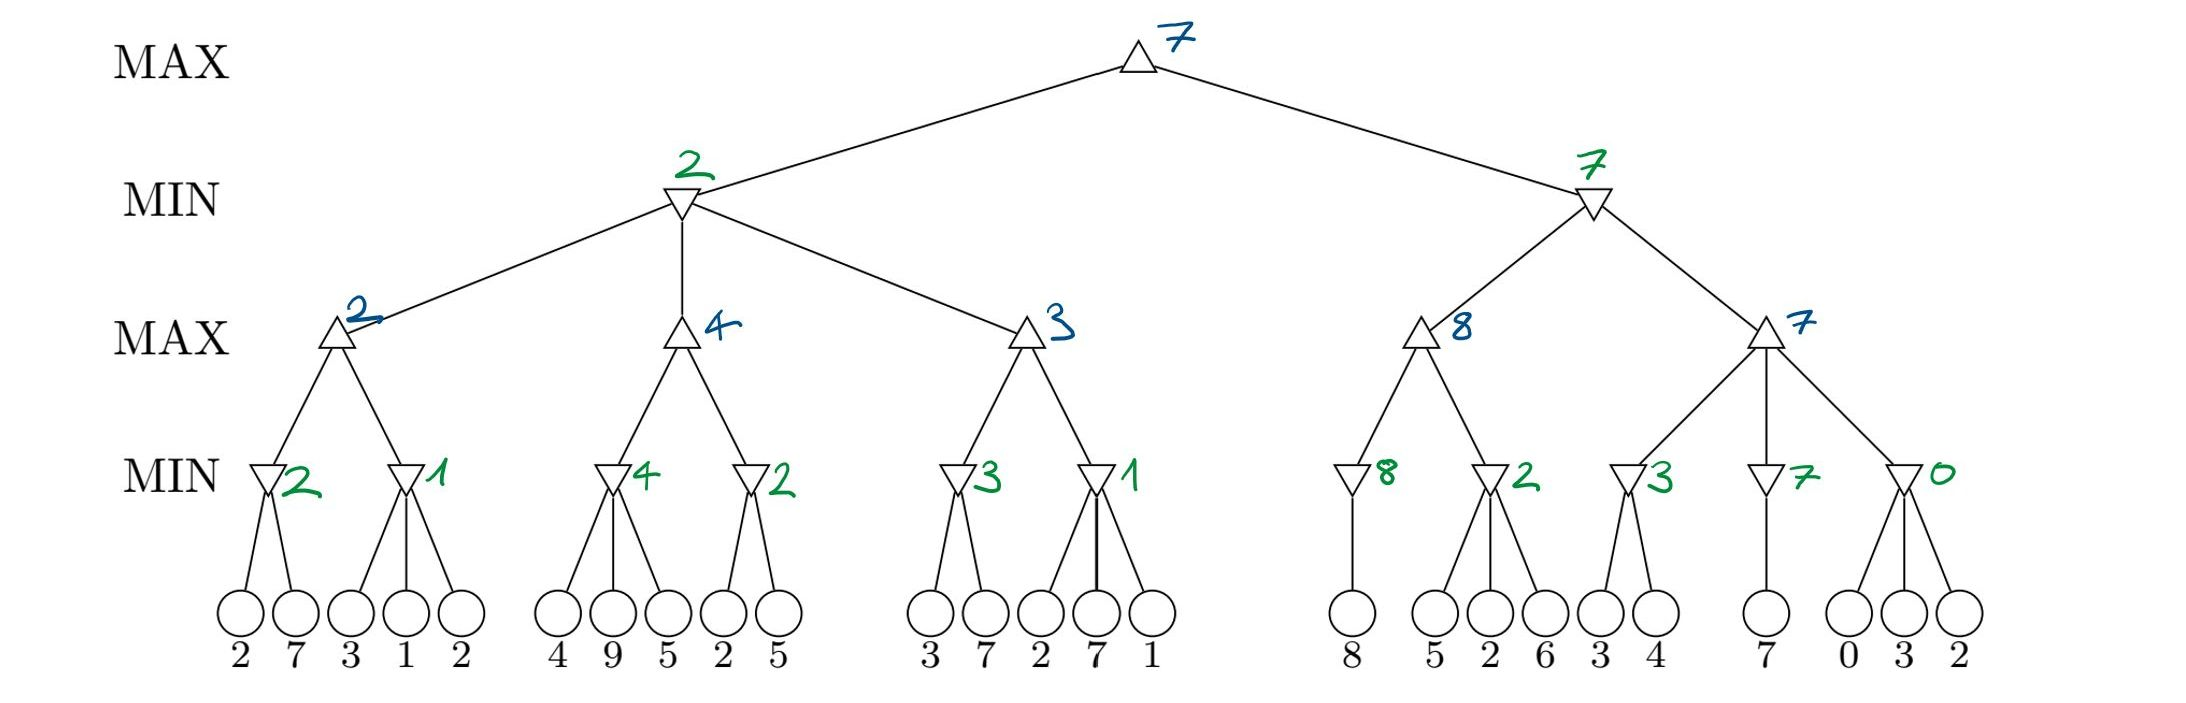
\includegraphics[width=0.99\linewidth]{assets/11_2_a.jpg}
    \end{figure}
    \item If both players play optimally, the obtained value will
    be 7 (see root node).
    The following plan will be chosen:
    \begin{figure}[!ht]
        \centering
        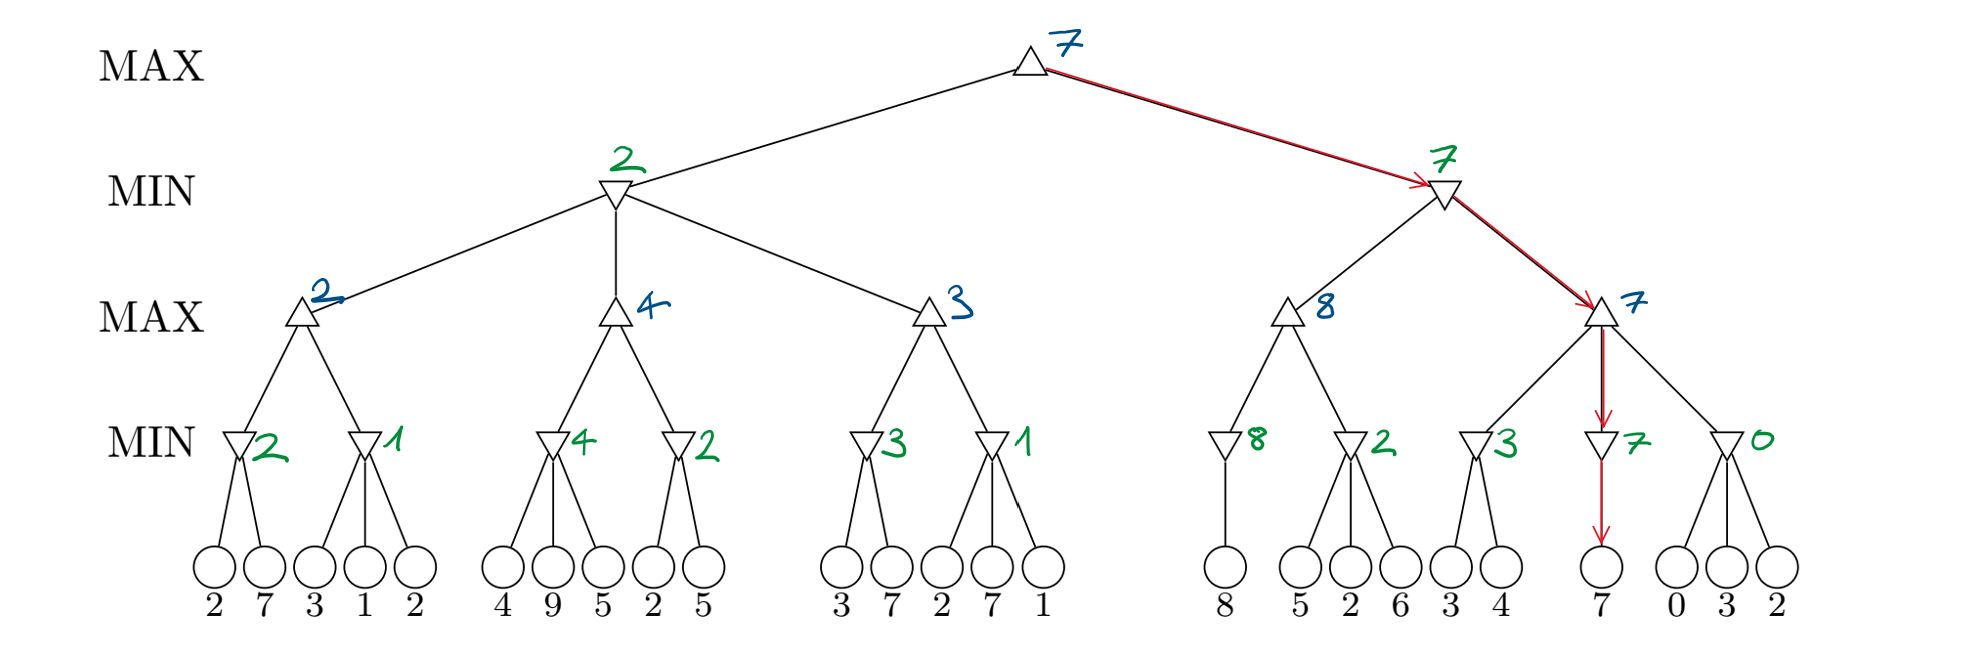
\includegraphics[width=0.99\linewidth]{assets/11_2_b.jpg}
    \end{figure}
    \item TODO
    \item TODO
\end{enumerate}

\section{}

\section{}

\section*{Statement on scientific integrity}
\begin{itemize}
    \item ChatGPT was asked for help with the definition of
    triangle nodes and the level distances in the game tree in 1(b)
\end{itemize}
Apart from that, we solved all exercises on our own.

\end{document}
